\chapter{Modelling and Simulation}

\graphicspath{{./Figures/Modeling}}

In this pivotal chapter, we meticulously derive the center of gravity and the moment of inertia for the two-wheeled self-balancing robot. These parameters are the linchpins of our dynamic analysis, serving as the critical variables within the equations of motion that govern the robot's behavior. By calculating these values with precision, we can substitute them into our dynamic equations, thereby tailoring the model to reflect the true dynamics of the robot. This process not only enhances the accuracy of our simulations but also ensures that the control strategies developed are based on a robust and representative model of the robot's physical capabilities. The careful derivation of these parameters is a testament to the thoroughness of our approach, ensuring that the resulting model is both reliable and predictive of the robot's real-world performance.
\newpage

\section{Mathematical Modelling}
\begin{itemize}
	\item \textbf{TWIPR Model:} Explanation of the Two-Wheeled Inverted Pendulum Robot (TWIPR) model.
	\item \textbf{Focus on 2D Dynamics:} Discussion on the scope limited to 2D dynamics and plans for future expansion to 3D dynamics and controller synthesis.
	\item \textbf{Assumptions and Parameters:} Detailing assumptions such as considering motor angles as parameters.
	\item \textbf{Model Derivation for \textit{l\_cg} and \textit{I\_y}:} Derivation of the models for center of gravity length (\textit{l\_cg}) and inertia around the y-axis (\textit{I\_y}).
	\item \textbf{Integration into TWIPR Model:} Integration of derived models into a new TWIPR framework.
	\item \textbf{Linear Model Derivation:} Derivation of the linear model from the integrated TWIPR model.
	
	$\bullet$ Modeling allows for predictive analysis and understanding of the robot's behavior.
	
	In order to predict the behavior of the robot under different settings, the modeling procedure entails constructing mathematical representations of the robot's dynamics and control systems.
	
	
	
	\begin{figure}[h]
		\centering
		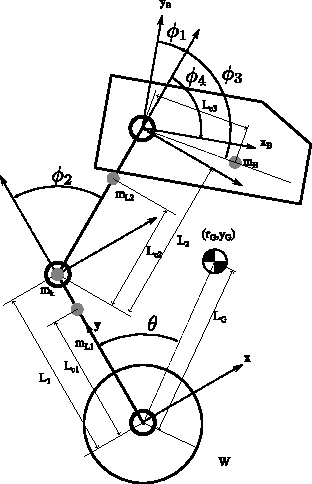
\includegraphics[width=.5\textwidth]{/Model}
		\caption[Mechanical model with the local coordinate system]{Figure illustrating the mechanical model with the local coordinate system to determine the center of gravity.}
		\label{Mechanical model with the local coordinate system}
	\end{figure}
	
	%Center of Gravity
	Center of Gravity calculations 
	\subsection{Center of Gravity } 
	$\bullet$ in that section the calculations of the overall center of gravity 
	
	$\bullet$ Significance in Dynamics:The stability of an object is directly impacted by the COG position, which also affects how it reacts to forces and moments from the outside world.
	
	$\bullet$ maintain equilibrium, 
	
	$\bullet$ accurately determining the COG is crucial for predicting and controlling dynamic behavior
	
	
	in the above figure in order to simplify the deriviation of the center of 
	
	\begin{equation}
		\begin{aligned}
			x_{CG} = \frac{m_{L1} \cdot 0 + m_K \cdot 0 + m_{L2} \cdot L_{C2} \cdot \sin(\phi_2) + m_B \cdot (L_2 \cdot \sin(\phi_2) + L_{C3} \cdot \sin(\phi_2 + \phi_3))}{m_{L1} + m_{L2} + m_K + m_B}
		\end{aligned}
	\end{equation}
	
	\begin{equation}
		\begin{aligned}
			y_{CG} = \frac{m_{L1} \cdot L_{C1} + m_K \cdot L_1 + m_{L2} \cdot (L_1 + L_{C2} \cdot \cos(\phi_2)) + m_B \cdot (L_1 + L_2 \cdot \cos(\phi_2) + L_{C3} \cdot \cos(\phi_2 + \phi_3))}{m_{L1} + m_{L2} + m_K + m_B}
		\end{aligned}
	\end{equation}
	
	%\begin{equation}
	%\begin{aligned}
	%	x_{CG} &= \frac{{m_{L1} L_{C1} \sin(\phi_1) + m_K L_1 \sin(\phi_1) + m_{L2} (L_1 \sin(\phi_1) + L_{C2} \sin(\phi_2 - \phi_1))}}{m_{L1} + m_{L2} + m_K + m_B} \nonumber \\
	%	&\quad + \frac{m_B (L_1 \sin(\phi_1) + L_2 \sin(\phi_2 - \phi_1) + L_{C3} \sin(\phi_3 + \phi_2 - \phi_1))}{m_{L1} + m_{L2} + m_K + m_B}
	%\end{aligned}
	%\end{equation}
	%
	%\begin{equation}
	%\begin{aligned}
	%	y_{CG} &= \frac{{m_{L1} L_{C1} \cos(\phi_1) + m_K L_1 \cos(\phi_1) + m_{L2} (L_1 \cos(\phi_1) + L_{C2} \cos(\phi_2 - \phi_1))}}{m_{L1} + m_{L2} + m_K + m_B} \nonumber \\
	%	&\quad + \frac{m_B (L_1 \cos(\phi_1) + L_2 \cos(\phi_2 - \phi_1) +L_{C3} \cos(\phi_3 + \phi_2 - \phi_1))}{m_{L1} + m_{L2} + m_K + m_B}
	%\end{aligned}
	%\end{equation}
	
	\begin{equation}
		L_G = \sqrt{x_{CG}^2 + y_{CG}^2}
	\end{equation}
	
	\begin{equation}
		\theta = \arctan\left(\frac{{x_{CG}}}{{y_{CG}}}\right)
	\end{equation}
	
	
	\begin{figure}[h]
		\centering
		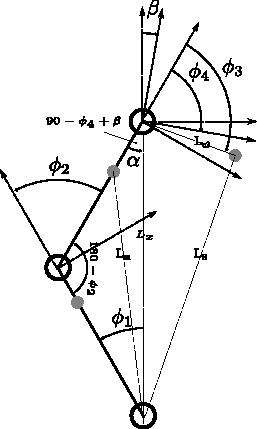
\includegraphics[width=.5\textwidth]{/Angles}
		\caption[Moment of inertia Schematic representation]{Schematic representation detailing the requisite angles and lengths for calculating the moment of inertia.}
		\label{fig:Schematic representation detailing the requisite angles and lengths for calculating the moment of inertia.}
	\end{figure}
	
	\subsection{Moment of inertia}
	%MOI
	Moment of inertia calculations 
	\begin{equation}
		L_m = \sqrt{L_1^2 + L_{C2}^2 - L_1 L_{C2} \cos(180 - \phi_2)}
	\end{equation}
	
	\begin{equation}
		L_{x} = \sqrt{L_1^2 + L_2^2 - L_1 L_2 \cos(180 - \phi_2)}
	\end{equation}
	
	
	\begin{equation}
		\alpha = \cos^{-1} \left( \frac{l_2^2 + l_{x}^2 - l_1^2}{2 l_2 l_{x}} \right) 
	\end{equation}
	
	%\begin{equation}
	%	\alpha = 90 - \phi_4 + \beta
	%\end{equation}
	
	\begin{equation}
		L_b = \sqrt{L_{x}^2 + L_{C3}^2 - Lx L_{C3} \cos(180 - \alpha - \phi_3 )}
	\end{equation}
	
	\begin{equation}
		I_{L1} = \frac{1}{12} m_{L1} (a_1^2 + b_1^2)
	\end{equation}
	\begin{equation}
		I_{L2} = \frac{1}{12} m_{L1} (a_2^2 + b_2^2)
	\end{equation}
	\begin{equation}
		I_K = \frac{1}{2} m_K R_m^2
	\end{equation}
	\begin{equation}
		I_B = \frac{1}{12} m_B (a_B^2 + b_B^2)
	\end{equation}
	\begin{equation}
		I = I_{L1} + m_{L1} L_{C1}^2 + I_K + m_K L_1^2 + I_{L2} + m_{L2} L_m^2 + I_B + m_B L_b^2
	\end{equation}
	
	\subsection{Equation of motion }
	%equation of motion 
	Equation of motion 
	
	
	
	
	
	
	\subsection{Dynamics of the Two-Wheeled Inverted Pendulum Robot}
	Given the functions $B_i: \mathbb{R} \rightarrow \mathbb{R}$, $C_{ij}: \mathbb{R} \rightarrow \mathbb{R}$, $D_{ij}: \mathbb{R} \rightarrow \mathbb{R}$, and $V_i: \mathbb{R} \rightarrow \mathbb{R}$, $i,j \in \{1,2,3\}$, the equations of motion are given by:
	
	\begin{align}
		\ddot{s} &= \frac{\sin(\Theta)}{V_1(\Theta)} \left( -C_{11}(\Theta) + C_{12}\dot{\Theta}^2 + C_{13}(\Theta)\dot{\psi}^2 \right) - \frac{D_{11}(\Theta)}{V_1(\Theta)}\dot{s} + \frac{D_{12}(\Theta)}{V_1(\Theta)}\dot{\Theta} + \frac{B_{1}(\Theta)}{V_1(\Theta)}(\tau_L + \tau_R) \\
		\ddot{\Theta} &= \frac{\sin(\Theta)}{V_1(\Theta)} \left( C_{21} - C_{22}(\Theta)\dot{\Theta}^2 - C_{23}(\Theta)\dot{\psi}^2 \right) + \frac{D_{21}(\Theta)}{V_1(\Theta)}\dot{s} - \frac{D_{22}(\Theta)}{V_1(\Theta)}\dot{\Theta} - \frac{B_{2}(\Theta)}{V_1(\Theta)}(\tau_L + \tau_R)  \\
		\ddot{\psi} &= \frac{\sin(\Theta)}{V_2(\Theta)} \left( C_{31}(\Theta)\dot{\Theta}\dot{\psi} - C_{32}(\Theta)\dot{\psi}\dot{s} \right) - \frac{D_{33}(\Theta)}{V_2(\Theta)}\dot{\psi} - \frac{B_{3}}{V_2(\Theta)}(\tau_L - \tau_R)
	\end{align}
	
	
	The equations of motion are derived in [44]. The functions $B_i: \mathbb{R} \rightarrow \mathbb{R}$, $C_{ij}: \mathbb{R} \rightarrow \mathbb{R}$, $D_{ij}: \mathbb{R} \rightarrow \mathbb{R}$, and $V_i: \mathbb{R} \rightarrow \mathbb{R}$, $i,j \in \{1,2,3\}$, are given by:
	
	\begin{equation}
		C_{11}(\Theta) = m_B^2 l^2 \cos(\Theta),
	\end{equation}
	\begin{equation}
		C_{12} = (I_2 + m_B l^2) m_B l,
	\end{equation}
	\begin{equation}
		C_{13}(\Theta) = (I_2 + m_B l^2) m_B l + m_B l (I_3 - I_1 - m_B l^2) \cos^2(\Theta),
	\end{equation}
	\begin{equation}
		C_{21} = (m_B + 2m_W + \frac{2J}{r^2}) m_B l,
	\end{equation}
	\begin{equation}
		C_{22}(\Theta) = m_B^2 l^2 \cos(\Theta),
	\end{equation}
	\begin{equation}
		C_{23}(\Theta) = m_B^2 l^2 + (m_B + 2m_W + \frac{2J}{r^2}) (I_3 - I_1 - m_B l^2) \cos(\Theta).
	\end{equation}
	\begin{equation}
		C_{31}(\Theta) = 2 (I_3 - I_1 - m_B^2) \cos(\Theta),
	\end{equation}
	\begin{equation}
		C_{31} = m_B l,
	\end{equation}
	\begin{equation}
		D_{11}(\Theta) = \frac{(I_2 + m_B^2) 2c_\alpha}{r^2} - \frac{m_B \cos(\Theta) 2c_\alpha}{r},
	\end{equation}
	\begin{equation}
		D_{12}(\Theta) = \frac{(I_2 + m_B^2) 2c_\alpha}{r} - 2m_B \cos(\Theta) c_\alpha,
	\end{equation}
	\begin{equation}
		D_{21}(\Theta) = \frac{(m_B + 2m_W + \frac{2J}{r^2}) 2c_\alpha}{r} + \frac{m_B \cos(\Theta) 2c_\alpha}{r^2},
	\end{equation}
	\begin{equation}
		D_{22}(\Theta) = \frac{(m_B + 2m_W + \frac{2J}{r}) 2c_\alpha + m_B \cos(\Theta) 2c_\alpha}{r},
	\end{equation}
	\begin{equation}
		D_{33}(\Theta) = \frac{d^2}{2r^2 c_\alpha},
	\end{equation}
	\begin{equation}
		B_{1} = \frac{(I_2 + m_B^2) \frac{1}{r} + m_B \cos(\Theta)}{r},
	\end{equation}
	\begin{equation}
		B_{2} = \frac{m_B l}{r} - \cos(\Theta) + m_B + 2m_W + \frac{2J}{r^2},
	\end{equation}
	\begin{equation}
		B_{3} = \frac{d}{2r},
	\end{equation}
	\begin{equation}
		V_{1} = (m_B + 2m_W + \frac{2J}{r^2}) (I_2 + m_B^2) - m_B^2 \cos^2(\Theta),
	\end{equation}
	\begin{equation}
		V_{2} = I_3 + 2K + (m_W + \frac{J}{r^2}) \frac{d^2}{2} - (I_3 - I_1 - m_B^2) \sin^2(\Theta).
	\end{equation}
	
	
	\begin{table}[h!]
		\centering
		\caption{Parameters of the mechanical system}
		\label{tab:parameters}
		\begin{tabular}{lcl}
			\toprule
			Parameter & Value & Description \\
			\midrule
			$m_B$ & 2.5 kg & mass of the pendulum body \\
			$m_W$ & 0.636 kg & mass of a wheel \\
			$l$ & 0.026 m & distance between the wheel axis and the pendulum's center of gravity \\
			$d$ & - & distance between the two wheels \\
			$J$ & \(5.175 e^{-4}\) kgm\textsuperscript{2} & moment of inertia of a wheel w.r.t. reference frame \{C\} in direction of \(c_2\) \\
			$K$ & - & moment of inertia of a wheel w.r.t. reference frame \{C\} in direction of \(c_3\) \\
			$I_1$ & - & moment of inertia of pendulum's body w.r.t. reference frame \{B\} in direction of \(b_1\) \\
			$I_2$ & \(0.0165\) kgm\textsuperscript{2} & moment of inertia of pendulum's body w.r.t. reference frame \{B\} in direction of \(b_2\) \\
			$I_3$ & - & moment of inertia of pendulum's body w.r.t. reference frame \{B\} in direction of \(b_3\) \\
			$c_\alpha$ & \(4.630 e^{-4}\) Nms & viscous friction coefficient \\
			\bottomrule
		\end{tabular}
	\end{table}
\end{itemize}

\section{Numerical Simulation}
\begin{itemize}
	\item \textbf{Discrete Numerical Simulation:} Elaboration on the process of discrete numerical simulation, including the discrete double integration method to arrive at the state vector.
\end{itemize}

\section{Simulation Environment}
\begin{itemize}
	\item \textbf{Overview of the Simulation Environment:} A brief overview of the simulation environment, referencing David's Bachelor Thesis for details.
	
	
	\item \textbf{Integration of the Model:} Description of integrating the new TWIPR model into the simulation environment and a summary of the individual components of the model.
\end{itemize}

\section{Controller Synthesis}
\begin{itemize}
	\item \textbf{State-Space Controllers:} Introduction to two state-space controllers: Linear Quadratic Regulator (LQR) and Pole-Placement.
	\item \textbf{Configuration Specificity:} Explanation of how these controllers are specific to one configuration (knee angle and hip angle) of the robot.
	\item \textbf{Controller Retuning Algorithm:} Presentation of an algorithm for retuning the controllers as the configuration changes.
\end{itemize}

\section{Simulation Analysis}
\begin{itemize}
	\item \textbf{Controller Responses:} Analysis of step response and responses to other inputs using one of the controllers in different configurations.
	\item \textbf{Impact of Non-Retuning:} Discussion on the effects of not retuning the controllers.
	\item \textbf{Influence of Leg Configuration:} Analysis of how leg configuration influences the robot's behavior.
	\item \textbf{Controller Setting Comparisons:} Comparative study of different controller settings and a comparison between LQR and Pole-Placement controllers.
	\item \textbf{Optimal Controller Configuration:} Conclusion on which controller configuration might be best suited for such a robot.
\end{itemize}










	


